\section{Solution Framework}

This section details how the proposed hybrid PT/DT architecture is \emph{realized} across two mission phases: (i) \textbf{deployment-time initialization} (mission geometry, initial conditions, DT thresholds and policies) and (ii) \textbf{operation-time execution} (local PT control, exception reporting, DT predictive simulation, and spare staging). We focus on distributed control, event-driven messaging, and resilience logic.

\subsection{PT Distributed Control and Local Sensing}

Each physical asset (PT) operates as an autonomous agent, executing a distributed density-balancing algorithm based on local sensing. The control law combines:
\begin{itemize}
    \item \textbf{Mission force:} Drives the asset toward its next assigned waypoint.
    \item \textbf{Repulsive force:} Maintains safe separation from neighboring assets within detection radius $r_d$.
    \item \textbf{Spacing force:} Adjusts speed to correct for local spacing anomalies.
\end{itemize}

%Let $i$ denote the current asset, and $n$ its neighbors. The control law is as follows:
%\begin{align}
%\text{neighbors} &\gets \text{DetectNeighbors}(r_d) \label{eq:neighbors} \\
%d_{\text{fwd}} &\gets \text{ArcDistanceFwd}(i, n) \label{eq:dfwd} \\
%d_{\text{back}} &\gets \text{ArcDistanceBack}(i, n) \label{eq:dback} \\
%s_{\text{avg}} &\gets (d_{\text{fwd}} + d_{\text{back}})/2 \label{eq:savg} \\
%\text{error} &\gets s_{\text{avg}} - s_{\text{nominal}} \label{eq:error}
%\end{align}

The virtual forces are:
%\begin{align}
%F_{\text{mission}} &= k_m \cdot \text{DirectionTo}(\text{waypoint}_{\text{current}}) \label{eq:fmission} \\
%F_{\text{repulsion}} &= \sum_{n \in \text{neighbors}} f_{\text{rep}}(i, n) \label{eq:frep} \\
%F_{\text{spacing}} &= 
%\begin{cases}
%k_s \cdot \text{error} \cdot \text{TangentDirection}(), & |\text{error}| > \epsilon \\
%0, & \text{otherwise}
%\end{cases} \label{eq:fspacing}
%\end{align}

%where $f_{\text{rep}}(i, n) = k_r \cdot \frac{d_{\text{safe}} - d}{d^2} \cdot (\text{position}_i - n.\text{position})$ if $d < d_{\text{safe}}$, and $0$ otherwise.

The velocity update is:
%\begin{align}
%F_{\text{total}} &= F_{\text{mission}} + F_{\text{repulsion}} + F_{\text{spacing}} \label{eq:ftotal} \\
%v_{\text{desired}} &= F_{\text{total}} / m_i \label{eq:vdesired} \\
%v_i &\gets \text{Clamp}(v_{\text{desired}}, v_{\min}, v_{\max}) \label{eq:vclamp} \\
%v_i &\gets \alpha v_i + (1-\alpha) v_{\text{prev}} \label{eq:vsmooth}
%\end{align}
Rebalancing is required whenever the fleet's structure evolves, such as after a loss event or the insertion of new assets (feeding). As previously mentioned, loss events—along with intrusion detection—are the primary cases where the system's furtivity is momentarily and deliberately broken to enable exception reporting and strategic intervention.

\subsection{Event-Driven Messaging Protocol}

When a PT detects a significant event (e.g., loss, intrusion, anomaly), it sends an event message:
\begin{equation}
m_i^t = \langle t,\, \mathbf{x},\, \text{type},\, \text{source\_id},\, c \rangle
\label{eq:msg}
\end{equation}
where $t$ is the event timestamp, $\mathbf{x}$ is the location, $\text{type}$ indicates the event class, $\text{source\_id}$ identifies the reporting asset, and $c$ is an optional confidence score.

  extbf{A perimeter intrusion} event is detected when an intruder is classified as \emph{inside} the patrolled polygon.

\paragraph{Intrusion identification (point-in-polygon via ray casting, $\mathcal{O}(n)$).}
Each drone knows its own position $\mathbf{x}_i^t$ and the ordered waypoint set $\mathcal{W}=\{\mathbf{w}_1,\dots,\mathbf{w}_n\}$ defining the perimeter polygon. When an intruder is perceived at $\mathbf{y}^t$, the drone classifies it using a standard \emph{ray casting} test: it casts a ray from $\mathbf{x}_i^t$ to $\mathbf{y}^t$ and counts how many polygon edges it intersects. An odd number of intersections implies that $\mathbf{y}^t$ lies inside the polygon, and even implies outside.

Let $\chi(\mathbf{x}_i^t,\mathbf{y}^t,\mathcal{W})\in\{0,1\}$ denote the resulting inside-test (1 if inside). The computational cost is linear in the number of polygon edges, i.e., $\mathcal{O}(n)$.

If $\chi=1$, the drone emits an intrusion event:
\begin{equation}
m_i^t \equiv \langle t,\, \mathbf{y}^t,\, \text{intrusion},\, i,\, c_{i}^t \rangle.
\label{eq:intrusion_event}
\end{equation}
with confidence computed, for instance, as a decreasing function of the distance to the perimeter:
\begin{equation}
c_{i}^t = f\big(d(\mathbf{y}^t, \partial\mathcal{P})\big)
\label{eq:conf_intrusion}
\end{equation}
where $\partial\mathcal{P}$ denotes the polygon boundary.
\textbf{A loss  } event is detected when  a previously sensed neighbor $j$ is no longer detected:
\begin{align*}
& \forall i,\, \exists j \in Detected_i^{t-1} \ \&\  j \notin Detected_i^t \\
&\implies 
m_i^t \equiv \langle t,\, \mathbf{x}_j^{t-1},\, \text{loss},\, i,\, c_{i,j}^t \rangle
\label{eq:loss}
\end{align*}
with confidence:
\begin{equation}
c_{i,j}^t =  \frac{range_i - |x_i^{t-1} - x_j^{t-1}|}{range_i}
\label{eq:conf}
\end{equation}
 

\subsection{Digital Twin (DT) Monitoring: Suppletive and Reactive Modes}

The Digital Twin (DT) operates in two distinct modes, as illustrated in Figs.~\ref{fig:timeline_high_level} and~\ref{fig:timeline_zoom}:

\paragraph{Nominal (Suppletive) Mode}
In nominal conditions, the DT operates in \emph{suppletive} mode: it maintains an a priori model of the fleet and stays \emph{communication-silent} and \emph{compute-frugal}. In particular, it does not require continuous telemetry nor does it issue commands. The DT is only (re)activated when an exception event is reported by a PT asset, at which point it synchronizes and runs predictive what-if analyses. This low-emission stance is depicted in Fig.~\ref{fig:timeline_high_level}. 

\paragraph{Reactive (Predictive/Decision) Mode}
 

%At the Digital Twin (DT) level, fleet state updates are performed in an event-driven manner. Rather than continuously simulating all drone trajectories, the DT maintains a ``frozen'' internal state between exception events (such as a loss or intrusion). 
When a new event is received at time $t_j$, the DT analytically advances the positions of all drones from the last known state at $t_i$ by applying a shift of $(t_j - t_i) \bmod T_{\text{lap}}$, where $T_{\text{lap}} = p/v$ is the patrol period for perimeter length $p$ and nominal speed $v$. This efficient update mechanism, illustrated in Fig.~\ref{fig:timeline_zoom}, allows the DT to instantly synchronize its internal model with the real fleet state upon event arrival, without the computational overhead of step-by-step integration. This stands in contrast to the design-phase pure simulation, which continuously integrates the dynamics of all assets for exhaustive exploration, and to the physical twin, which operates in real time. The DT’s analytic, event-driven update is a key enabler for scalable, low-overhead fleet supervision, as discussed in \ref{subsec:distinguishing}.

Once synchronized, the DT transitions to reactive mode. It then initiates a predictive simulation over an adaptation window $T_{\text{adapt}}$, using the same distributed control law as the PT to forecast the fleet’s response. The DT evaluates resilience and coverage metrics to determine whether self-adaptation is sufficient or if spare deployment is required. If any of the following conditions are met,
Once synchronized, the DT transitions to reactive mode. It then initiates a predictive simulation over an adaptation window $T_{\text{adapt}}$, using the same distributed control law as the PT to forecast the fleet’s response. The DT evaluates resilience and coverage metrics to determine whether self-adaptation is sufficient or if spare deployment is required. For \textbf{intrusion} events, the reporting drone may request \textbf{cross-confirmation} from a nearby PT (second viewpoint) before escalating to the DT, in order to reduce false alarms; such confirmation is not required for \textbf{loss/destruction} events, which already rely on neighborhood disappearance. If any of the following conditions are met,
\begin{align}
\sigma^2_{\rho,\text{pred}} &> \sigma^2_{\text{max}} \\
C_{\min} &< C_{\text{critical}} \\
n &< n_{\text{min}}
\end{align}
the DT computes an optimal insertion point (e.g., midpoint of the largest gap) and stages a spare asset. This event-driven activation and intervention process is illustrated in Fig.~\ref{fig:timeline_zoom}.

This architecture ensures that the DT only activates when necessary, preserving communication parsimony and operational stealth during routine operation, while enabling rapid, informed intervention when disruptions occur.

\subsection{Spare Self-Insertion Mechanism (Tooling-Independent)}
\label{subsec:spare_insertion}
This subsection describes the \emph{mechanism} by which a spare joins the circulation. It is a controller-level and architecture-level construct (independent of any specific simulator, middleware, or prototyping framework): the DT may provide a single \emph{insertion waypoint} to the spare, and the spare subsequently self-inserts using only local sensing.

To preserve furtivity and autonomy-first principles, spare drones are incorporated without broadcasting commands to the PT fleet. From the PT perspective, the spare appears as a new neighbor and is absorbed through the baseline density-balancing law.

\paragraph{Initialization-only logic.}
The spare runs a dedicated initialization routine \emph{prior} to joining the circulation. Once inserted, it switches to the exact same baseline PT code as all other drones (CR$^\circ$3: code uniformity). Convergence is achieved through the existing balancing dynamics.

\paragraph{State machine.}
The insertion routine is organized into four modes:
\begin{enumerate}
  \item \textbf{Approach}: navigate to the DT-provided insertion waypoint (or a default rendezvous waypoint).
  \item \textbf{Capture}: detect the circulation direction and acquire two nearest neighbors (front/back) using local sensing.
  \item \textbf{Insert}: regulate tangential speed to converge to the midpoint of the local gap while enforcing safety distances (reverse balancing).
  \item \textbf{Assimilate}: switch permanently to the baseline PT density-balancing controller.
\end{enumerate}

\paragraph{Reverse balancing (gap-centering) control.}
In \textbf{Insert} mode, the spare computes the arc-length distances to its nearest neighbor ahead ($d_f$) and behind ($d_b$) along the circulation direction, and defines a centering error $e_c = d_f - d_b$. It then adjusts its tangential speed to drive $e_c \to 0$ while adding a repulsion term to avoid unsafe compression. A simple 1D speed law is:
\begin{equation}
v_{\text{sp}} \gets \mathrm{clip}\big(v_0 - k_c\, e_c + v_{\mathrm{rep}}(d_f,d_b),\; v_{\min},\; v_{\max}\big)
\label{eq:spare_speed_control}
\end{equation}
where $k_c>0$ is a centering gain and $v_{\mathrm{rep}}$ is a negative (decelerating) term that increases as $\min(d_f,d_b)$ approaches $d_{\mathrm{safe}}$.

\paragraph{Assimilation condition.}
The spare transitions to \textbf{Assimilate} when (i) it is approximately centered ($|e_c|\le\varepsilon_c$) and (ii) safety constraints hold ($d_f,d_b\ge d_{\mathrm{safe}}$) for a dwell time $T_{\mathrm{dwell}}$. After this point, the spare executes the baseline PT algorithm unchanged, and the fleet converges through its standard cascade balancing.

\subsection{Flow}
\begin{figure}[h]
    \centering
    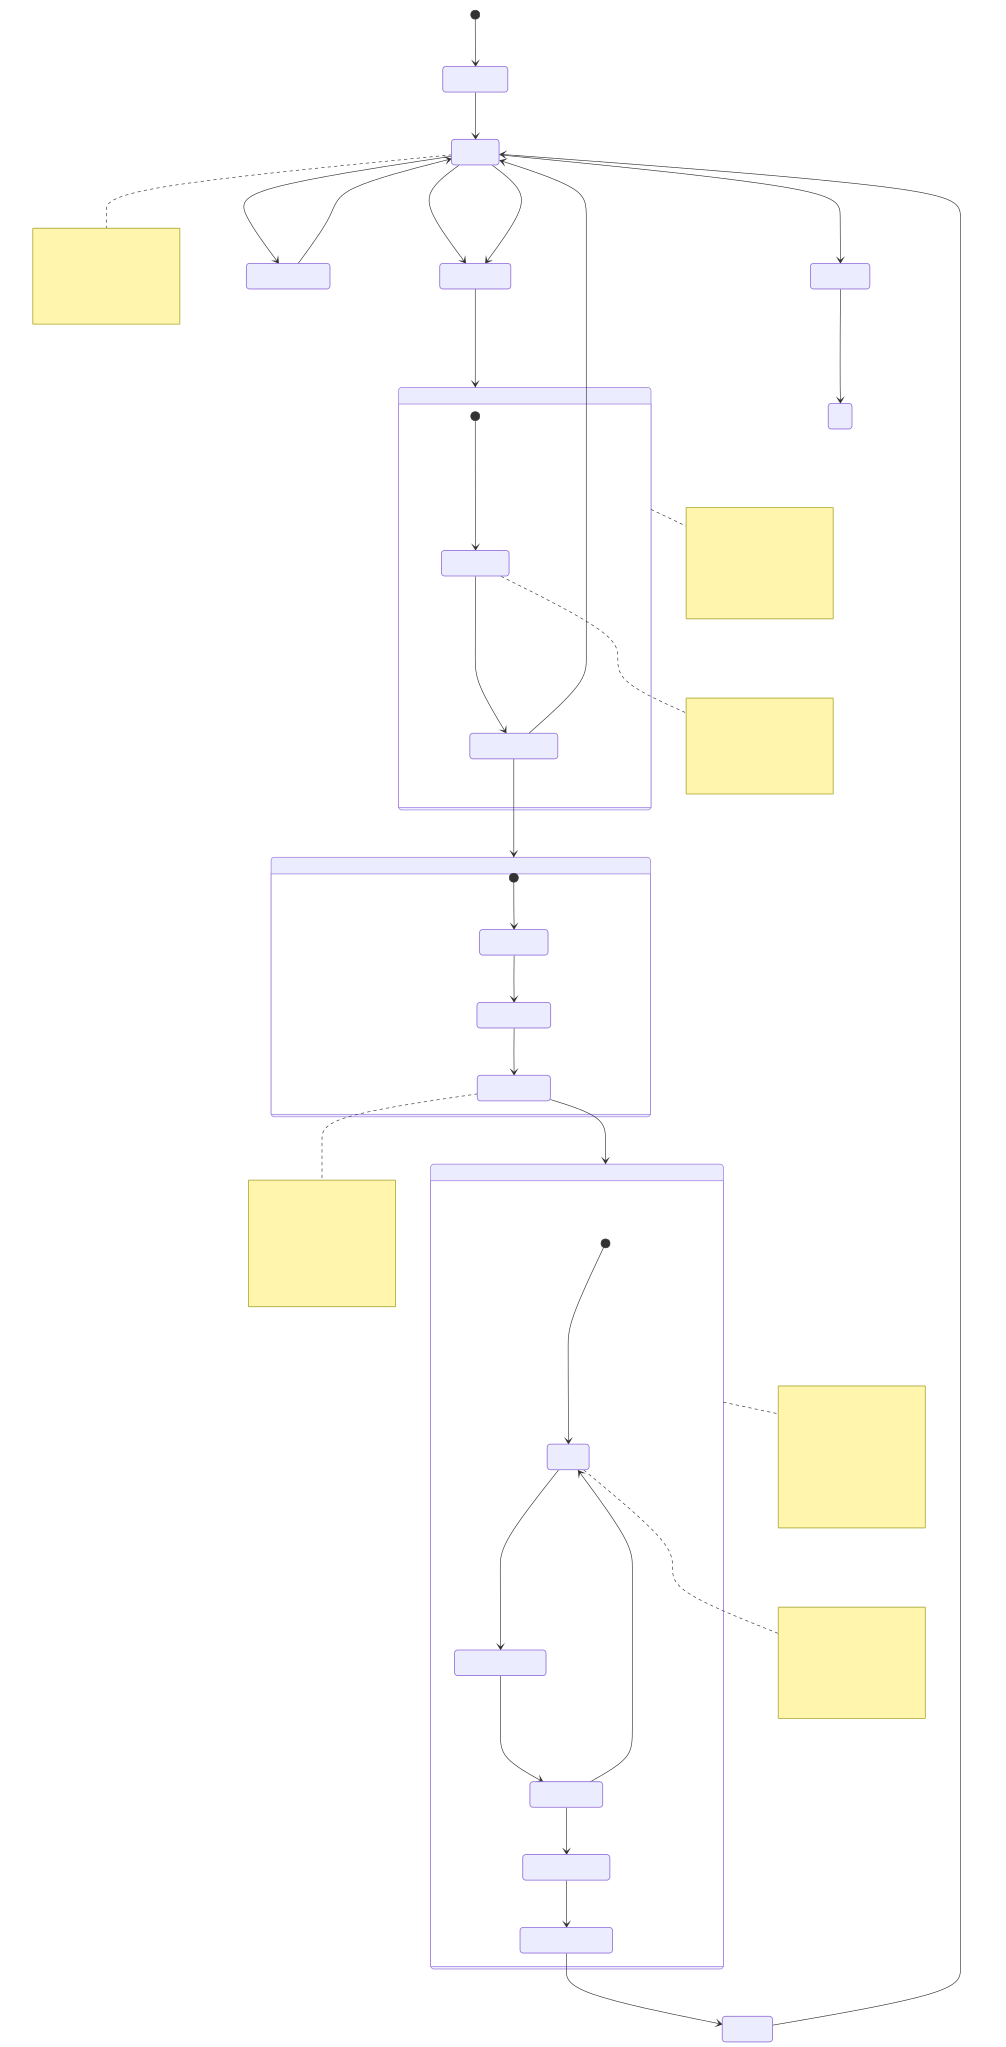
\includegraphics[width=0.95\linewidth]{figures/State-Drones.png}
    \caption{Drone Fleet System State Machine: PT+DT Orchestration}
    \label{fig:state_machine}
\end{figure}